% The Failure Is a Vector — diagnosis-first paper, SmolVLA / LIBERO-spatial.
% Self-contained article class with ICLR-like geometry so it compiles anywhere;
% swap to iclr20XX_conference.sty for the actual submission.
\documentclass{article}
\usepackage[margin=1in]{geometry}
\usepackage{times}
\usepackage{amsmath,amssymb,amsthm}
\usepackage{graphicx}
\usepackage{booktabs}
\usepackage{subcaption}
\usepackage{xcolor}
\usepackage[numbers,sort&compress]{natbib}
\usepackage[colorlinks=true,linkcolor=blue,citecolor=blue,urlcolor=blue]{hyperref}
\usepackage{cleveref}
\usepackage{microtype}

% Shared notation for the reach-field diagnostic.
\newcommand{\R}{\mathbb{R}}
\newcommand{\Ev}{\mathbf{E}}      % reach endpoint
\newcommand{\Cv}{\mathbf{C}}      % canonical (training) object location
\newcommand{\Tv}{\mathbf{T}}      % displaced true object location
\newcommand{\dv}{\mathbf{d}}      % displacement T - C
\newcommand{\ev}{\mathbf{e}}      % endpoint error E - T
\newcommand{\cossim}{\operatorname{cos}}
\newcommand{\proj}{\operatorname{proj}}
\newcommand{\smolvla}{SmolVLA}


\title{Anchored, Not Steered:\\ What Controls the Reach of a Competent SmolVLA Under Object Displacement}
\author{Anonymous Authors}
\date{}

\begin{document}
\maketitle

\begin{abstract}
Vision-language-action (VLA) policies fall into a ``memory trap'' under object displacement: when a manipulated object is moved from its training configuration the policy fails, and prior work has shown qualitatively that the end-effector is driven toward the object's original location. We ask a causal question that observing the failure cannot answer: \emph{what information actually controls the failed reach?} We pair a displacement-relative \emph{reach-field} diagnostic, which quantifies the endpoint error vector $\ev=\Ev-\Tv$ via $\cossim(\ev,-\dv)$ (positive $=$ reaching toward the canonical training location $\Cv$), with a \emph{renderer-local object-paste} intervention that holds the physical scene fixed and moves only the target object's rendered appearance---the counterfactual prior work does not run. On a competent SmolVLA checkpoint ($74\%$ clean success on LIBERO-spatial), (i) a $50$\,mm displacement leaves the reach endpoint anchored to the canonical location (clean-conditioned median $\cossim(\ev,-\dv)=0.759$, task-cluster bootstrap CI $[0.693,0.847]$, normalized projection $0.98$) while displaced success collapses to $31\%$, quantifying and confirming the memory trap; and (ii) across a $740$-rollout object-paste grid, grasp success tracks the \emph{physical} object position and is indifferent to the \emph{visual} one---showing the object at a displaced location leaves success essentially unchanged ($72\%$ vs.\ $75\%$ sham), while physically displacing it collapses success to ${\sim}31\%$ regardless of where it is shown, and the endpoint shift toward the pasted location is null ($S_{CT}=0.06$, $95\%$ CI $[-0.02,0.12]$). The bias is stable as competence rises from $60\%$ to $74\%$, and both findings replicate on a second LIBERO suite (LIBERO-object), where the bias is if anything stronger ($\cossim(\ev,-\dv)=0.97$). The competent policy's reach is anchored to a canonical endpoint prior and is not sufficiently steered by either the physical or the locally rendered object position, locating the displacement failure in the action prior rather than in local visual object localization.

\end{abstract}

\section{Introduction}
\label{sec:intro}

Vision-language-action (VLA) policies report strong success rates on standard manipulation benchmarks, yet a high aggregate success rate can hide brittle behavior under small, task-relevant changes to the scene. A policy that grasps a bowl on $74\%$ of unperturbed episodes may nonetheless fail when the same bowl is moved a few centimeters---a change a competent agent should absorb. Recent work has shown that such displacement-induced failures exist for VLA policies and framed them as a ``memory trap'' \citep{afi2025memorytrap}, showing qualitatively that the end-effector is driven toward the object's original location. We take that phenomenon as established and ask the next, \emph{causal} question---one that observing the failure cannot answer: \emph{what information actually controls the failed reach?}

A displacement failure could arise from (i) perception that mislocalizes the object, (ii) an inability to recover once the reach is underway, or (iii) a learned prior that aims at a fixed, canonical location largely independent of the current object position. These imply different remedies---better object localization, closed-loop recovery, or reshaping the action prior---yet success-rate metrics, and even the qualitative observation that the hand goes to the original location, cannot distinguish them. The distinguishing experiment is a \emph{counterfactual}: hold the physical scene fixed and change only where the object \emph{appears}.

\paragraph{Approach.} We run exactly that counterfactual. A \emph{renderer-local object-paste} intervention moves only the target object's rendered appearance to a chosen visual location while leaving its true pose, the rest of the scene, and the physics unchanged, so we can ask whether the reach follows the object's appearance or ignores it. We pair this active probe with a passive \emph{reach-field} measurement: after displacing the object by $\dv=\Tv-\Cv$ (with a fresh observation), we record the endpoint error $\ev=\Ev-\Tv$ and summarize it with $\cossim(\ev,-\dv)$ and the signed projection $\langle\ev,-\dv\rangle/\lVert\dv\rVert^2$ (near $0$ $=$ tracking the displaced object; near $1$ $=$ reaching back to the canonical location).

\paragraph{Contributions.}
\begin{itemize}
\item \textbf{Causal dissociation (main result).} Using a renderer-local object-paste counterfactual that prior work does not run, we show that a competent SmolVLA's reach endpoint is \emph{not sufficiently steered by the local rendered object position}: with the object physically canonical but shown displaced, it still grasps at the canonical location in $16/16$ trials, and the reverse paste does not rescue a displaced grasp (\cref{sec:sufficiency}). The displacement failure is located in the action prior, not in local visual object localization.
\item \textbf{Quantifying the memory trap.} We introduce a displacement-relative reach-field statistic and use it to confirm and \emph{quantify} the qualitative memory trap of \citet{afi2025memorytrap} on a competent ($74\%$) checkpoint: median $\cossim(\ev,-\dv)=0.759$ at $50$\,mm, monotonically increasing with displacement, with displaced success collapsing to $31\%$ (\cref{sec:competent}).
\item \textbf{Stability and generalization.} The bias holds across the full fine-tuning checkpoint ladder as clean success rises from $60\%$ to $74\%$ (so it is not an undertraining artifact), replicates across two training seeds, and replicates---more strongly---on a second LIBERO suite, LIBERO-object (\cref{sec:emergence,sec:generalization}).
\end{itemize}

\cref{fig:cloud} sets up the picture: under a $50$\,mm displacement the reach endpoints of a competent policy cluster at the canonical location $\Cv$, not the displaced object $\Tv$ (\cref{sec:competent}); the object-paste counterfactual (\cref{sec:sufficiency}) then shows this reach does not move \emph{even when the object's appearance does}. The remainder of the paper formalizes the diagnostic (\cref{sec:protocol}), quantifies the memory trap on a competent policy (\cref{sec:competent}), runs the causal counterfactual that is our main result (\cref{sec:sufficiency}), characterizes the bias's persistence across competence (\cref{sec:emergence}), and discusses implications and scope (\cref{sec:discussion,sec:limitations}).

\section{Related Work}
\label{sec:related}

\paragraph{Vision-language-action policies.} A growing family of VLA models maps language and visual observations to robot actions, typically by fine-tuning a vision-language backbone with an action head: RT-2 \citep{brohan2023rt2}, OpenVLA \citep{kim2024openvla}, $\pi_0$ \citep{black2024pi0}, and SmolVLA \citep{shukor2025smolvla}, the compact flow-matching policy we study. These models are usually evaluated by aggregate task success on benchmarks such as LIBERO \citep{liu2023libero}. Our work is orthogonal to model design: we take a published policy and recipe as given and ask what its failures \emph{look like} geometrically, rather than proposing a new architecture or training objective.

\paragraph{Displacement robustness and the memory trap.} Closest to us, \citet{afi2025memorytrap} introduce a displacement protocol and show that VLA policies suffer a ``memory trap'': they fail when a manipulated object is moved from its training configuration. \citet{liberopro2025} similarly probe robustness of LIBERO-trained policies under controlled perturbations. We treat the displacement phenomenon and its protocol as established by this line of work---AFI already shows qualitatively that the hand is driven toward the original location. Our contribution is not to re-discover that failure, but (i) to \emph{quantify} its endpoint geometry with a displacement-relative reach field on a demonstrably competent policy, and (ii) to run a \emph{counterfactual AFI does not}: holding the physical object fixed while changing only its rendered position, testing whether the local rendered object position is sufficient to steer the reach. Where prior work observes the failure under physical displacement, we causally dissociate the rendered object position from the reach endpoint---a distinction the qualitative observation ``ignoring new spatial cues'' leaves open.

\paragraph{Action representation and equivariance.} Our intervention design exploits the translation behavior of relative (delta) action policies, for which observation-frame translations compose with the action map in a known way \citep{wang2025equivariant}. We use this equivariance only as an off-the-shelf property to justify leaving the wrist channel untouched in early intervention variants; we do not claim it as a contribution. More broadly, action-diffusion and flow-matching policies \citep{chi2023diffusion,black2024pi0,shukor2025smolvla} produce action \emph{chunks} rather than single steps, which shapes how we define and measure the reach endpoint.

\paragraph{Diagnostic and causal evaluation of policies.} Beyond aggregate success, a body of work probes \emph{why} learned controllers behave as they do through targeted perturbations and interventions. Our renderer-local object-paste probe is in this spirit: rather than translating the whole observation frame---which we find to be out-of-distribution for the policy and therefore confounded---we move only the target object's rendered appearance, so the intervention isolates the agentview object channel without changing the rest of the scene. To our knowledge, applying such a local, content-preserving visual intervention to dissociate the reach endpoint from object position in a VLA policy is new; we position it as a diagnostic tool rather than a claim about all policies.

\section{Diagnostic Protocol}
\label{sec:protocol}

\paragraph{Policy and training.} We study SmolVLA \citep{shukor2025smolvla}, a compact flow-matching VLA, fine-tuned on LIBERO-spatial \citep{liu2023libero}. Following the standard SmolVLA full action-expert preset, we freeze the vision-language backbone and fine-tune the action expert (the only trainable module; $\sim$100M of 450M parameters) on all $432$ demonstrations across the $10$ tasks, for $100$k steps at learning rate $10^{-4}$ with a cosine schedule (warmup $1000$, decay over the full run to $2.5\times10^{-6}$), batch size $32$, in bfloat16. Actions are relative (delta) end-effector poses plus a gripper command, executed in chunks of $50$.

\paragraph{Clean evaluation (competence).} We measure clean success on a fixed, position-disciplined grid: each (task, seed) pair is rolled out in a freshly constructed environment with the object at its canonical location, for $10$ tasks $\times$ $5$ seeds $=50$ rollouts, using the standard LIBERO success criterion. We use clean success as the policy's \emph{competence}, the quantity a strong checkpoint must establish before any failure it exhibits can be attributed to the policy rather than to undertraining.

\paragraph{Reach-field protocol.} For a displacement of magnitude $m$ in a cardinal direction, we move the target object from its canonical location $\Cv$ to $\Tv=\Cv+\dv$ at episode start and re-render the observation so the policy plans on the post-displacement image (we verified that a naive observation refresh returns a cached, pre-displacement frame; all reach-field rollouts force a fresh render). We then roll out the policy and record three endpoint definitions of the end-effector trajectory: the \emph{pregrasp} endpoint (pose at first gripper closure), the \emph{closest} approach to the object, and the \emph{final} pose. The \emph{primary} endpoint is pregrasp where defined, else closest. All endpoints are taken in the table ($xy$) plane, the plane of displacement.

\paragraph{Clean-conditioned primary set.} Our primary analysis conditions on \emph{clean-success pairs}: displaced rollouts whose paired clean rollout (same (task, seed), same run) succeeded. This is the direct answer to the ``weak/undertrained policy'' objection---the policy provably solves the undisplaced task, so any displacement failure is not an inability to do the task. Clean success defines $37$ of the $50$ task-seed pairs as clean-capable, so the $50$\,mm primary set comprises $37\times4=148$ displaced rollouts (one per cardinal direction per clean-capable pair); displaced success is reported separately over those displaced trials. We report all-attempt and clean-conditioned-failure subsets as secondary views.

\paragraph{Statistics.} For each displaced rollout we form the displacement $\dv=\Tv-\Cv$ and the endpoint error $\ev=\Ev-\Tv$, and report (i) the directional alignment $\cossim(\ev,-\dv)$ (positive $=$ reaching toward the canonical prior, zero $=$ tracking the displaced object), (ii) the signed projection $\langle\ev,-\dv\rangle/\lVert\dv\rVert^2$ (a magnitude-transfer measure: $1$ means the endpoint stays at $\Cv$ as the object moves), and (iii) the fraction of endpoints closer to $\Cv$ than to $\Tv$. Population summaries use the median with a \emph{task-cluster bootstrap} $95\%$ CI (resampling tasks, then pooling their rollouts) to respect the per-task correlation of canonical geometry. We pre-registered a replication bar (\cref{tab:protocol}); the pooled $|\ev|\!\sim\!|\dv|$ regression $R^2$ is reported descriptively only, as it is confounded by per-task geometry and is not a valid gate.

\begin{table}[t]
\centering
\caption{Protocols, sample sizes, primary metrics, and pre-registered pass bars.}
\label{tab:protocol}
\small
\begin{tabular}{@{}llll@{}}
\toprule
Protocol & Rollouts & Primary metric & Pass bar \\
\midrule
E0 clean eval & $50$ ($10{\times}5$) & clean success & strong ckpt $\geq 33/50$ ($65\%$) \\
E1r reach-field & $850$ ($50{\times}17$) & $\cossim(\ev,-\dv)$, $50$\,mm, clean-cond. & med.\ $\geq 0.50$; boot-low $>0.20$; \\
 & & & proj.\ $\geq 0.35$; closer-canon.\ $\geq 0.65$ \\
E2r object-paste & $740$ ($37{\times}4{\times}5$) & $S=\langle\Ev_{CT}{-}\Ev_{CC},\dv\rangle/\lVert\dv\rVert^2$ & sufficiency: med.\ $S\geq0.40$ \\
Emergence ladder & $4{\times}250$ & bias vs.\ competence & (descriptive) \\
\bottomrule
\end{tabular}
\end{table}

\section{A Competent Policy Still Fails Under Displacement}
\label{sec:competent}

\paragraph{The checkpoint is competent (E0).} The full action-expert fine-tune reaches $37/50=74\%$ clean success on the position-disciplined grid, with every task succeeding on at least one seed (per-task range $20$--$100\%$; median successful rollout length $104$ steps). This clears our pre-registered strong-checkpoint bar ($\geq 65\%$) and rules out the objection that the effect appears only in a weak $30$--$40\%$ policy. For comparison, a parameter-efficient (LoRA) fine-tune of the same backbone plateaus at $36$--$38\%$ regardless of learning rate; only the full action-expert recipe yields a competent policy (\cref{sec:emergence,sec:appendix}).

\paragraph{Displacement drives the reach to the canonical prior (E1r).} We run the full reach-field grid ($50$ pairs $\times$ $\{$clean $+$ $4$ magnitudes $\times$ $4$ cardinal directions$\}=850$ rollouts; $37$ clean-success pairs enter the primary set). At the headline $50$\,mm displacement, the clean-conditioned primary endpoint yields a median $\cossim(\ev,-\dv)=0.759$ with task-cluster bootstrap CI $[0.693,0.847]$, a signed projection of $0.98$, and $68\%$ of endpoints closer to the canonical location $\Cv$ than to the displaced object $\Tv$. All four pre-registered criteria pass. \cref{fig:cloud} shows the geometry directly: in the displacement frame, the endpoints of a competent policy form a cloud centered at $\Cv$, not at the object $\Tv$. A projection of $0.98$ means the endpoint barely moves as the object is displaced---the policy reaches as though the object were still at its training location. The effect replicates on an independent training seed (seed-1: $50$\,mm clean-conditioned median $\cossim(\ev,-\dv)=0.844$ at $76\%$ clean success, overlapping CI), so it is not a single-seed artifact (\cref{sec:limitations}).

\begin{figure}[t]
\centering
\begin{subfigure}{0.46\textwidth}
  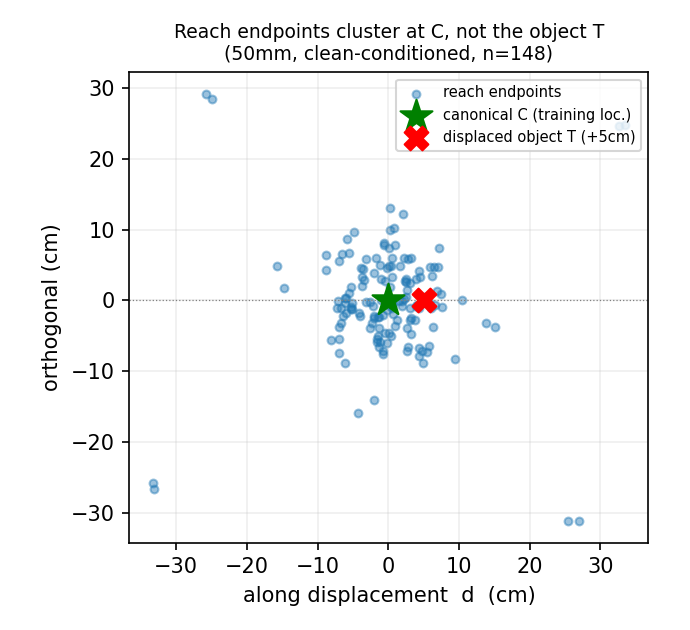
\includegraphics[width=\linewidth]{figures/fig_endpoint_cloud.png}
  \caption{Endpoints cluster at $\Cv$, not $\Tv$ ($50$\,mm).}
  \label{fig:cloud}
\end{subfigure}\hfill
\begin{subfigure}{0.46\textwidth}
  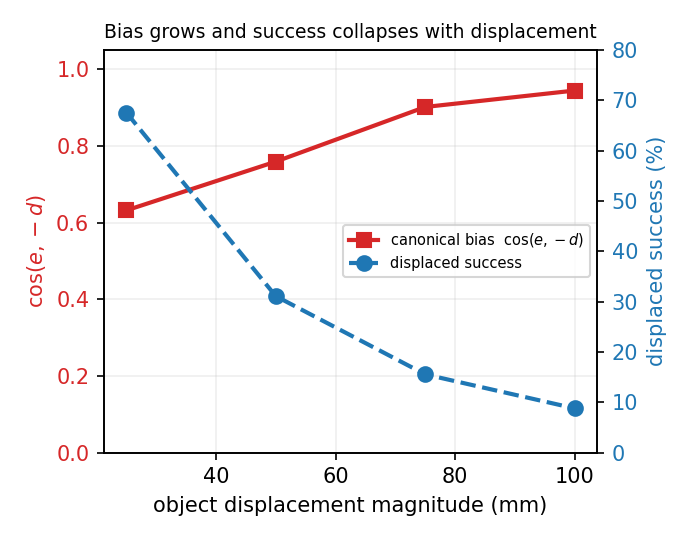
\includegraphics[width=\linewidth]{figures/fig_magnitude.png}
  \caption{Bias rises and success collapses with magnitude.}
  \label{fig:magnitude}
\end{subfigure}
\caption{\textbf{Reach-field on the competent ($74\%$) SmolVLA checkpoint.} (a) Clean-conditioned reach endpoints $\Ev$ in the displacement frame ($x$ along $\dv=\Tv-\Cv$); green star $=$ canonical/training location $\Cv$, red cross $=$ displaced object $\Tv$. The endpoint error is $\ev=\Ev-\Tv$, and our statistic $\cossim(\ev,-\dv)>0$ means the reach points back toward $\Cv$ (the canonical prior). (b) The alignment $\cossim(\ev,-\dv)$ increases monotonically with displacement while displaced success collapses.}
\label{fig:e1r}
\end{figure}

\paragraph{The bias scales and predicts failure.} The alignment increases monotonically with displacement magnitude---median $\cossim(\ev,-\dv)$ of $0.63$, $0.76$, $0.90$, $0.94$ at $25$, $50$, $75$, $100$\,mm---and the fraction closer to canonical rises from $61\%$ to $86\%$ (\cref{fig:magnitude}). In lockstep, displaced success collapses from $68\%$ at $25$\,mm to $31\%$, $16\%$, and $9\%$, despite $74\%$ clean success. The larger the displacement, the more the reach ignores it, and the more the episode fails. The endpoint error points toward the canonical prior \emph{despite a fresh post-displacement observation}: the policy is not acting on stale pixels, but on a location it has learned to aim at.

\section{Local Visual Object Position Is Not Sufficient}
\label{sec:sufficiency}

The reach-field result is correlational: under displacement, the reach points at $\Cv$. But \emph{why}? One hypothesis is that the agentview object position drives the endpoint, and displacement simply moves it out of a learned in-distribution band. If so, then \emph{showing} the object at a location should move the reach there. We test this with a causal intervention.

\paragraph{Renderer-local object paste.} A naive test---translating the entire observation frame---is itself out-of-distribution for the policy (in pilot runs a global frame translation broke $87\%$ of otherwise-healthy episodes), so it cannot cleanly adjudicate sufficiency. Instead we move only the object's \emph{appearance}: at each policy step we save the target object's pose, kinematically set it to a \emph{visual} location $V$, re-render the cameras, restore the true pose, and feed the policy the re-rendered image while stepping the real physics. This changes only the object's $\sim$2k rendered pixels (both agentview and wrist), leaving the rest of the scene---and the real physics---intact (a no-op sham render changes $0$ pixels, confirming the machinery is identity when $V$ equals the physical location).

\paragraph{Design.} We cross physical and visual object location in a $2{\times}2$ factorial plus a specificity control, at $50$\,mm on the clean-success pairs: \textbf{CC} (physical $\Cv$, visual $\Cv$; sham), \textbf{CT} (physical $\Cv$, visual $\Tv$; the primary sufficiency arm), \textbf{TC} (physical $\Tv$, visual $\Cv$), and \textbf{CR} (physical $\Cv$, visual $\Cv+R_{90}\dv$; a specificity control that pastes the object at an orthogonal $90^\circ$ visual displacement). The sufficiency statistic is the endpoint shift from sham toward the pasted location, $S=\langle\Ev_{CT}-\Ev_{CC},\dv\rangle/\lVert\dv\rVert^2$; $S\!\approx\!1$ means the reach follows the visually-pasted object, $S\!\approx\!0$ means it ignores it.

\paragraph{Visual position does not steer the reach.} Over the full $740$-rollout grid, showing the object at a false location does not move the reach (\cref{fig:e2r}). The endpoint shift toward the pasted location is null: $S_{CT}$ has median $+0.06$ (task-cluster bootstrap $[-0.02,+0.12]$), only $32\%$ of CT endpoints are closer to the visually-pasted $\Tv$ than to $\Cv$, and the orthogonal specificity control is likewise inert ($S_{CR}=-0.04$). The success pattern is decisive and precision-independent: grasp success tracks the \emph{physical} object position and is indifferent to the \emph{visual} one. With the object physically at $\Cv$, showing it displaced barely changes success (\textbf{CT} $72\%$, $106/148$, vs.\ sham \textbf{CC} $75\%$, $111/148$); with the object physically at $\Tv$, showing it back at $\Cv$ does not help (\textbf{TC} $30\%$, $44/148$, vs.\ \textbf{TT} $32\%$, $48/148$). In \textbf{CT} the policy grasps the object at its true canonical location despite seeing it elsewhere---if the rendered position steered the reach, CT would aim at $\Tv$ and fail. The reach endpoint is thus decoupled from the agentview object position, both its real and its visually-pasted value.

\begin{figure}[t]
\centering
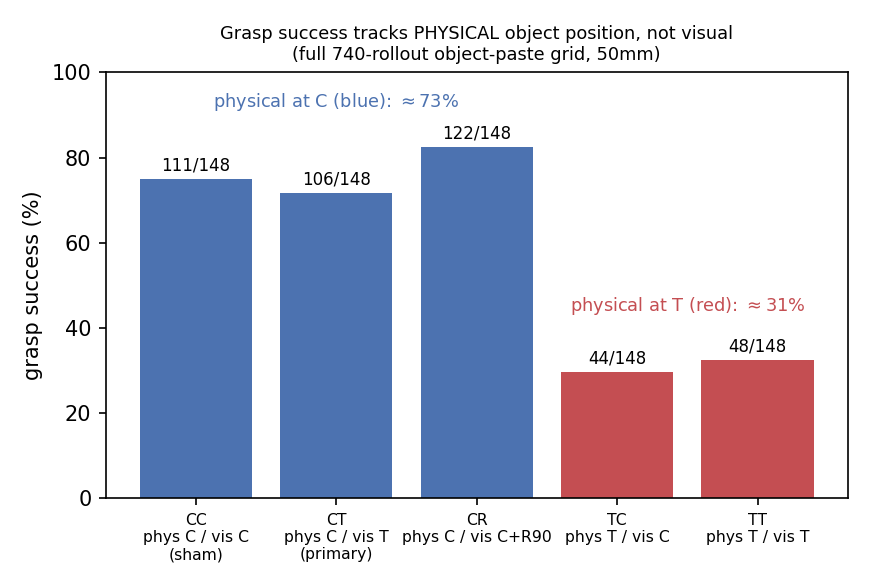
\includegraphics[width=0.55\textwidth]{figures/fig_e2r.png}
\caption{\textbf{Object-local paste intervention (full $740$-rollout grid, $50$\,mm).} Grasp success by condition (counts above bars), colored by \emph{physical} object location. Success tracks the physical position (at $\Cv$: CC/CT/CR $\approx 73$--$82\%$; at $\Tv$: TC/TT $\approx 30\%$) and is indifferent to the \emph{visual} position: CT (physical $\Cv$, shown $\Tv$) $\approx$ sham CC, and TC (physical $\Tv$, shown $\Cv$) $\approx$ TT. Showing the object elsewhere does not move the hand there.}
\label{fig:e2r}
\end{figure}

\paragraph{Interpretation.} Taken with \cref{sec:competent}, two manipulations that place the object's appearance away from $\Cv$---a real displacement (E1r) and a visual paste to a false location (CT)---both leave the reach endpoint aimed at $\Cv$, while pasting a displaced object's appearance back at $\Cv$ (TC) fails to rescue the displaced physical task. The endpoint is consistent with a canonical prior decoupled from the current agentview object position, rather than tracking it. We reserve the ``not sufficient'' claim to exactly this intervention: local rendered object position does not steer the reach in this setting. The CT-vs-TC success contrast is decisive independent of endpoint precision.

\section{The Bias Persists Across Competence}
\label{sec:emergence}

If the canonical-prior bias were a symptom of undertraining, it should weaken as the policy improves. We test this by running a reduced reach-field ($50$\,mm, $4$ directions, $250$ rollouts) at four points along the full action-expert training trajectory ($10$k, $40$k, $70$k, $100$k steps), recovering both axes from each run: clean success (competence) and the clean-conditioned bias $\cossim(\ev,-\dv)$.

\paragraph{Bias is stable across the checkpoint ladder.} Across this full action-expert ladder, as clean success rises from $60\%$ to $74\%$, the bias stays flat, $\cossim(\ev,-\dv)\in[0.76,0.82]$, with the closer-to-canonical fraction in $[68\%,74\%]$ (\cref{fig:ladder}; per-checkpoint values in \cref{tab:ladder}). More training does not erode the bias---if anything it is marginally lower at the most competent checkpoint, within noise. The mislocalization is therefore stable as this policy becomes more competent over the measured range, not a transient artifact that more training within this trajectory removes.

\begin{figure}[t]
\centering
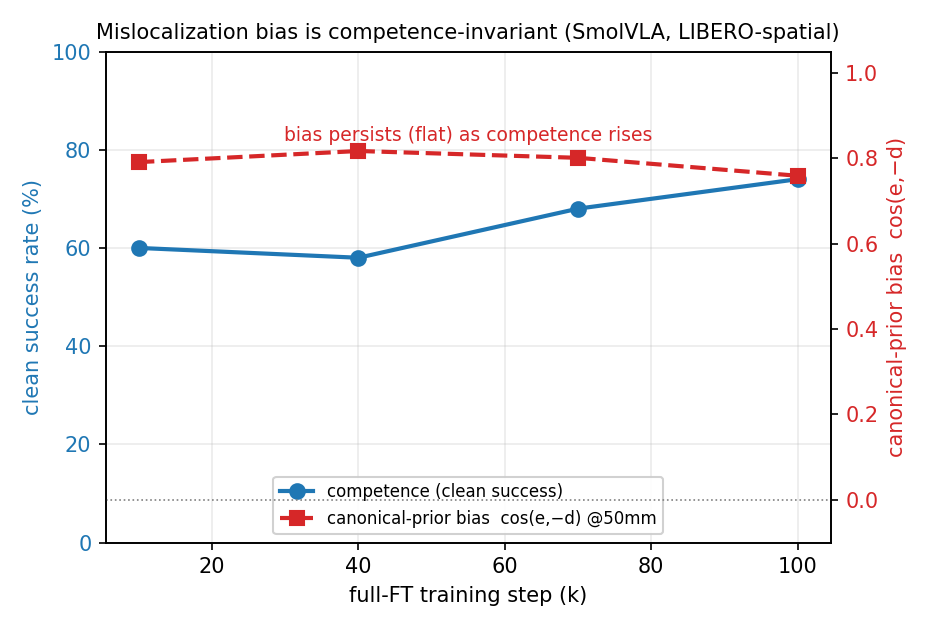
\includegraphics[width=0.55\textwidth]{figures/fig_ladder.png}
\caption{\textbf{Bias vs.\ competence along training.} As clean success rises ($60\!\to\!74\%$, blue), the canonical-prior bias $\cossim(\ev,-\dv)$ stays flat ($\sim\!0.78$, red). The failure mode does not diminish with competence.}
\label{fig:ladder}
\end{figure}

\begin{table}[t]
\centering
\caption{Emergence ladder (full action-expert checkpoints, $50$\,mm, clean-conditioned).}
\label{tab:ladder}
\small
\begin{tabular}{@{}lcccc@{}}
\toprule
Checkpoint & FT-10k & FT-40k & FT-70k & FT-100k \\
\midrule
Competence (clean success) & $60\%$ & $58\%$ & $68\%$ & $74\%$ \\
Bias $\cossim(\ev,-\dv)$ & $0.79$ & $0.82$ & $0.80$ & $0.76$ \\
Closer-to-canonical & $72\%$ & $74\%$ & $71\%$ & $68\%$ \\
\bottomrule
\end{tabular}
\end{table}

\paragraph{Caveat.} The competence range here is compressed: full action-expert fine-tuning is already $60\%$ competent by $10$k steps, so this ladder cannot probe the very-low-competence regime within the same recipe. We read it as evidence that the bias does not vanish as a competent policy gets \emph{more} competent, not as a claim about the full $0\!\to\!100\%$ competence axis (which would require mixing recipes and thereby confound competence with optimization).

\section{Generalization to a Second Suite}
\label{sec:generalization}

To test whether the canonical-prior reach is specific to LIBERO-spatial, we repeat the core protocol on \textbf{LIBERO-object}: a separate full action-expert checkpoint (same recipe, $68\%$ clean success), the E1r reach-field at $50$\,mm, and the E2 paste conditions (\cref{tab:suites}). Both findings replicate, and more strongly. The reach-field bias is sharper (median $\cossim(\ev,-\dv)=0.971$, $91\%$ of endpoints closer to canonical, vs.\ $0.759$/$68\%$ on spatial)---consistent with LIBERO-object's canonical object positions being tightly fixed across seeds, so the memorized reach target is sharper. The dissociation is also starker: showing the object displaced barely changes success (CT $79\%$ vs.\ CC $71\%$), but physically displacing it while showing it at canonical collapses success to $3\%$ (TC), with a null endpoint-steering coefficient ($S_{CT}=0.00$). The canonical-prior reach, and its decoupling from local visual object position, is therefore not specific to one LIBERO suite.

\begin{table}[t]
\centering
\caption{The canonical-prior reach and its visual decoupling replicate across two LIBERO suites.}
\label{tab:suites}
\small
\begin{tabular}{@{}lcc@{}}
\toprule
 & LIBERO-spatial & LIBERO-object \\
\midrule
Clean success (competence) & $74\%$ & $68\%$ \\
E1r $50$\,mm clean-cond.\ median $\cossim(\ev,-\dv)$ & $0.759$ $[0.69,0.85]$ & $0.971$ $[0.91,0.98]$ \\
\quad closer-to-canonical & $68\%$ & $91\%$ \\
E2 success: CC / CT / TC & $75 / 72 / 30\%$ & $71 / 79 / 3\%$ \\
\bottomrule
\end{tabular}
\end{table}

\section{Discussion}
\label{sec:discussion}

\paragraph{The failure is consistent with a canonical reach prior, not local-visual tracking.} The three results compose into a single account. The reach-field (\cref{sec:competent}) shows that under displacement the endpoint points to the canonical training location, with the alignment growing as the object moves further and the episode failing in proportion. The object-paste intervention (\cref{sec:sufficiency}) shows the local agentview object position is not sufficient to steer the endpoint: moving only the object's appearance does not move the reach, and the policy grasps the physically-present object even while shown it elsewhere. The emergence ladder (\cref{sec:emergence}) shows the bias is stable as competence rises. The parsimonious account is that the policy reaches toward a canonical location---where the object sat during training---largely insensitive to the current locally rendered object position. ``The failure is a vector'': it has a consistent direction (toward $\Cv$) and a magnitude that scales with displacement. We do not directly measure the policy's internal object estimate, so we frame this as a decoupling from the tested physical and local-visual positions rather than a claim about latent perception.

\paragraph{Relationship to prior work.} \citet{afi2025memorytrap} established that VLA policies fall into a memory trap under displacement and proposed remediation. We do not re-establish that failures occur; we quantify their endpoint geometry and localize their cause. The distinction matters for remedies: if displacement failures were purely a local-visual perception problem, better object localization or visual augmentation would help; our intervention suggests that, for this policy, the local agentview object position is not what the endpoint is tracking, so remedies targeting object localization alone may not suffice. Our results suggest remedies should also target action readout / prior formation---e.g., training distributions that decorrelate the reach target from a canonical location, or architectures that more tightly condition the action on current object state.

\paragraph{Implications for evaluation.} A $74\%$ clean-success policy that reaches the wrong location on $69\%$ of $50$\,mm displacements is invisible to aggregate success on the unperturbed benchmark. Reporting \emph{where} a policy reaches---a vector field, not a scalar---surfaces failure modes that scalar success hides, and does so with a cheap, model-agnostic probe (endpoints are already produced by any rollout). We suggest displacement-relative reach fields as a lightweight diagnostic to accompany success rates when evaluating VLA spatial robustness.

\section{Limitations and Scope}
\label{sec:limitations}

This study is intentionally diagnostic rather than benchmark-comprehensive. All experiments use SmolVLA-base, on two LIBERO suites (spatial and object); we do not test other VLA families, so the single-model scope is the main remaining boundary. The keystone replicates across two independent training seeds---seed-0 gives a $50$\,mm clean-conditioned median $\cossim(\ev,-\dv)=0.759$ (CI $[0.693,0.847]$) at $74\%$ competence, seed-1 gives $0.844$ (CI $[0.710,0.916]$) at $76\%$, with overlapping task-cluster intervals---so the effect is not a single-seed artifact, though two seeds remain a modest sample. We do not claim a tight point estimate of the paste-steering coefficient $S$, only that local rendered object position does not steer the reach. The emergence ladder spans a compressed competence range ($60$--$74\%$) because full action-expert fine-tuning is already competent by $10$k steps, so it speaks to invariance as a competent policy improves, not to the full competence axis. We therefore do not claim that all VLA families or robot embodiments exhibit the same vector field. The claim is bounded and falsifiable: for a competent SmolVLA policy on LIBERO-spatial and LIBERO-object, displacement failures are quantitatively explained by a canonical-prior reach field that is decoupled from local visual object position and stable across competence. Extending the diagnostic to a second VLA family (e.g., OpenVLA or $\pi_0$) is the natural next step for establishing cross-architecture generality.


\bibliographystyle{plainnat}
\bibliography{references}

\appendix
\section{Implementation and Reproducibility Details}
\label{sec:appendix}

\paragraph{Why full action-expert fine-tuning.} A parameter-efficient LoRA fine-tune (rank $64$, $\sim$3M trainable parameters) of the same SmolVLA backbone plateaus at $36$--$38\%$ clean success and does not clear the strong-checkpoint bar, independent of learning rate ($10^{-3}$ and the preset $10^{-4}$ give statistically indistinguishable results, $18/50$ and $19/50$). Only the full action-expert fine-tune (frozen vision-language backbone, $\sim$100M trainable parameters, $100$k steps) reaches $74\%$. We therefore use the full action-expert checkpoint as the competent policy throughout; the LoRA checkpoints serve only as low-competence references and are not the subject of any claim.

\paragraph{Fresh-observation discipline.} Robosuite's default observation accessor returns a cached frame that does not reflect direct object-pose mutation; an early version of the protocol planned the first post-displacement chunk on a stale, pre-displacement image. All reach-field and intervention rollouts force a fresh render after any pose change, so the policy always plans on the post-displacement (or post-paste) observation.

\paragraph{Endpoint extraction.} The pregrasp endpoint is the end-effector pose at the first gripper-close transition; the closest endpoint is the nearest approach (in the $xy$ plane) to the physical object; the final endpoint is the last pose. The primary endpoint is pregrasp where a gripper-close occurs, else closest. Cosine and projection statistics use the realized displacement $\dv$ (filtered to $\geq 1$\,cm) in the table plane.

\paragraph{Bootstrap.} Confidence intervals resample tasks with replacement (cluster bootstrap over the $10$ tasks), pool the resampled tasks' rollouts, and take the median; we report the $2.5$/$97.5$ percentiles over $10^4$ resamples.

\paragraph{Object-paste machinery.} Per policy step: save the target object's free-joint $qpos$; set its $xy$ to the visual location $V$; \texttt{sim.forward()} and re-render; restore $qpos$ and \texttt{sim.forward()}; feed the policy the re-rendered image(s) with the true proprioception, and step the real physics with the object at its physical location. Both the agentview and wrist images are edited. A sham render ($V$ equal to the physical location) changes $0$ pixels, confirming the intervention is identity in the no-op case; CT/TC/CR change only the $\sim$2k pixels of the object's footprint.

\paragraph{Reproducibility.} All result files (per-rollout endpoints, frozen verdict JSONs, and figures) and the harness scripts are released with the paper.


\end{document}
